
\documentclass[10pt]{beamer}
\usetheme{umbc2}
\useinnertheme{umbcboxes}
\setbeamercolor{umbcboxes}{bg=violet!12,fg=black}

\usepackage{longtable}
\usepackage{tabu}

\newcommand{\ul}{\underline}
\newcommand{\be}{\begin{equation}}
\newcommand{\ee}{\end{equation}}
\newcommand{\bdm}{\begin{displaymath}}
\newcommand{\edm}{\end{displaymath}}
\newcommand{\bea}{\begin{eqnarray}}
\newcommand{\eea}{\end{eqnarray}}
\newcommand{\bsea}{\begin{subeqnarray}}
\newcommand{\esea}{\end{subeqnarray}}
\newcommand{\mb}[1]{\mbox{#1}}
\newcommand{\mc}[3]{\multicolumn{#1}{#2}{#3}}
\newcommand{\bm}[1]{\mbox{\bf #1}}
\newcommand{\bmm}[1]{\mbox{\boldmath$#1$\unboldmath}}
\newcommand{\bmell}{\bmm\ell}
\newcommand{\hateps}{\widehat{\bmm\varepsilon}}
\newcommand{\graybox}[1]{\psboxit{box .9 setgray fill}{\fbox{#1}}}
\newcommand{\mdeg}[1]{\mbox{$#1^{\mbox{\scriptsize o}}$}}
\newcommand{\dd}{\mbox{\footnotesize{$\nabla \! \Delta$}}}
\newcommand{\p}{\partial\,}
\renewcommand{\d}{\mbox{d}}
\newcommand{\dspfrac}{\displaystyle\frac}
\newcommand{\nl}{\\[4mm]}

\title{Processing GNSS Data in Real-Time}

\author{Leo\v{s} Mervart}

\institute{TU Prague}

\date{Frankfurt, January 2014}

% \AtBeginSection[]
% {
%   \begin{frame}
%     \frametitle{Table of Contents}
%     \tableofcontents[currentsection]
%   \end{frame}
% }

\begin{document}

%%%%%%%%%%%%%%%%%%%%%%%%%%%%%%%%%%%%%%%%%%%%%%%%%%%%%%%%%%%%%%%%%%%%%%%%%%%%%%%%

\begin{frame}
  \titlepage
\end{frame}

%%%%%%%%%%%%%%%%%%%%%%%%%%%%%%%%%%%%%%%%%%%%%%%%%%%%%%%%%%%%%%%%%%%%%%%%%%%%%%%%

\begin{frame}
\frametitle{Medieval Times of GNSS (personal memories)}

\begin{description}
\item[1991] Prof. Gerhard Beutler became the director of the Astronomical Institute, University of
  Berne. The so-called Bernese GPS Software started to be used for (post-processing) analyzes of
  GNSS data.
\item[1992] LM started his PhD study at AIUB.
\item[1992] Center for Orbit Determination in Europe (consortium of AIUB, Swisstopo, BKG, IGN, and
  IAPG/TUM) established. Roughly at that time LM met Dr. Georg Weber for the first time.
\item[1993] International GPS Service formally recognized by the IAG.
\item[1994] IGS began providing GPS orbits and other products routinely (January, 1).
\item[1995] GPS declared fully operational.
\end{description}

\end{frame}

%%%%%%%%%%%%%%%%%%%%%%%%%%%%%%%%%%%%%%%%%%%%%%%%%%%%%%%%%%%%%%%%%%%%%%%%%%%%%%%%

\begin{frame}
\frametitle{CODE-Related Works in 1990's}

\begin{itemize}
\item The Bernese GPS Software was the primary tool for CODE analyzes (Fortran~77).
\item IGS reference network was sparse.
\item Real-time data transmission limited (Internet was still young, TCP/IP widely accepted 1989).
\item CPU power of then computers was limited (VAX/VMS OS used at AIUB).
\end{itemize}

In 1990's high precision GPS analyzes were almost exclusively performed in post-processing mode.
The typical precise application of GPS at that time was the processing of a network of static
GPS-only receivers for the estimation of station coordinates.

\end{frame}

%%%%%%%%%%%%%%%%%%%%%%%%%%%%%%%%%%%%%%%%%%%%%%%%%%%%%%%%%%%%%%%%%%%%%%%%%%%%%%%%

\begin{frame}
\frametitle{Tempora mutantur (and maybe ``nos mutamur in illis'')}

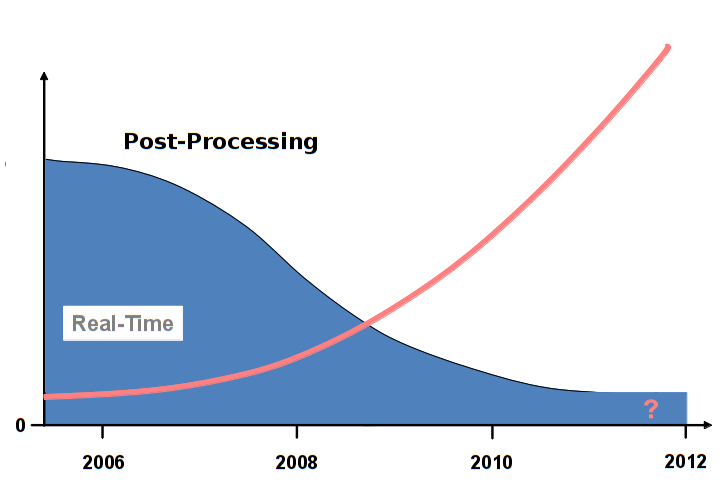
\includegraphics[width=0.7\textwidth,angle=0]{pp_vs_rt.png}

\vspace*{-2cm}
\hspace*{6cm}
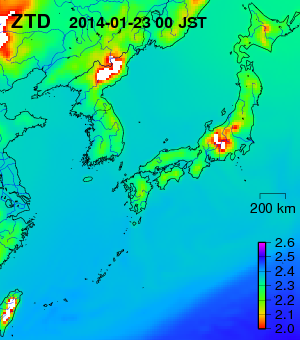
\includegraphics[width=0.4\textwidth,angle=0]{ea_ztd_21h.png}


\end{frame}


%%%%%%%%%%%%%%%%%%%%%%%%%%%%%%%%%%%%%%%%%%%%%%%%%%%%%%%%%%%%%%%%%%%%%%%%%%%%%%%%

\begin{frame}
\frametitle{O tempora! O mores!}

\begin{itemize}
\item people want more and more \ldots
\item everybody wants everything immediately \ldots
\item \hspace*{2cm} and, of course, free of charge \ldots
\end{itemize}
\vspace*{5mm}
In GNSS-world it means:
\begin{itemize}
\item There are many new kinds of GNSS applications - positioning is becoming just one of many
  purposes of GNSS usage.
\item Many results of GNSS processing are required in real-time (or, at least, with very small
  delay).
\item GPS is not the only positioning system. Other GNSS are being established (for practical but
  also for political reasons).
\item People are used that many GNSS services are available free of charge (but the development and
  maintenance has to be funded). 
\end{itemize}

\begin{block}{But \ldots}
\end{block}

\end{frame}

%%%%%%%%%%%%%%%%%%%%%%%%%%%%%%%%%%%%%%%%%%%%%%%%%%%%%%%%%%%%%%%%%%%%%%%%%%%%%%%%

\begin{frame}
\frametitle{Nihil novi sub sole}

Each GNSS-application is based on processing code and/or phase observations that may be expressed
as 
  \begin{eqnarray*}
  P^i & = & \varrho^i + c\;\delta - c\;\delta^i + T^i + I^i + b_P              \\
  L^i & = & \varrho^i + c\;\delta - c\;\delta^i + T^i - I^i + b^i
  \end{eqnarray*}
  where
  \begin{tabbing}
  $P^i$, $L^i$ ~~~~~~~ \= are the code and phase measurements, \\ 
  $\varrho^i$          \> is the travel distance between the satellite 
                          and the receiver,                               \\
  $\delta$, $\delta^i$ \> are the receiver and satellite clock errors,    \\
  $I^i$                \> is the ionospheric delay,                       \\
  $T^i$                \> is the tropospheric delay,                      \\
  $b_P$                \> is the code bias, and                           \\
  $b^i$                \> is the phase bias (including initial
                          phase ambiguity).
  \end{tabbing}


\end{frame}

%%%%%%%%%%%%%%%%%%%%%%%%%%%%%%%%%%%%%%%%%%%%%%%%%%%%%%%%%%%%%%%%%%%%%%%%%%%%%%%%

\begin{frame}

Observation equations reveal what information can be gained from processing GNSS data:
\begin{itemize}
\item geometry (receiver positions, satellite orbits), and
\item state of atmosphere (both dispersive and non-dispersive part)
\end{itemize}

The observation equations also show that, in principle, GNSS is an
\textcolor{blue!90}{interferometric} technique -- precise results are actually always relative.

\end{frame}

%%%%%%%%%%%%%%%%%%%%%%%%%%%%%%%%%%%%%%%%%%%%%%%%%%%%%%%%%%%%%%%%%%%%%%%%%%%%%%%%

\begin{frame}
\frametitle{Challenges of Real-Time GNSS Application}

\end{frame}

\end{document}
